\section{Anwendungsf�lle}
Anwendungsf�lle helfen fachlichen Anforderungen eines Systems darzustellen, indem dort Interaktionen zwischen System und Benutzer dargestellt werden.\newline
\begin{center}
 \begin{minipage}{\linewidth}
	\centering
	\includegraphics[scale=0.5]{../Bilder/UseCaseUebersicht.png}
	\captionof{figure}[kurze Bildunterschrift]{Bildunterschrift}
 \end{minipage}
\end{center}

\textbf{Anwendungsfall AF 1}
\begin{center}
 \begin{minipage}{\linewidth}
	\centering
	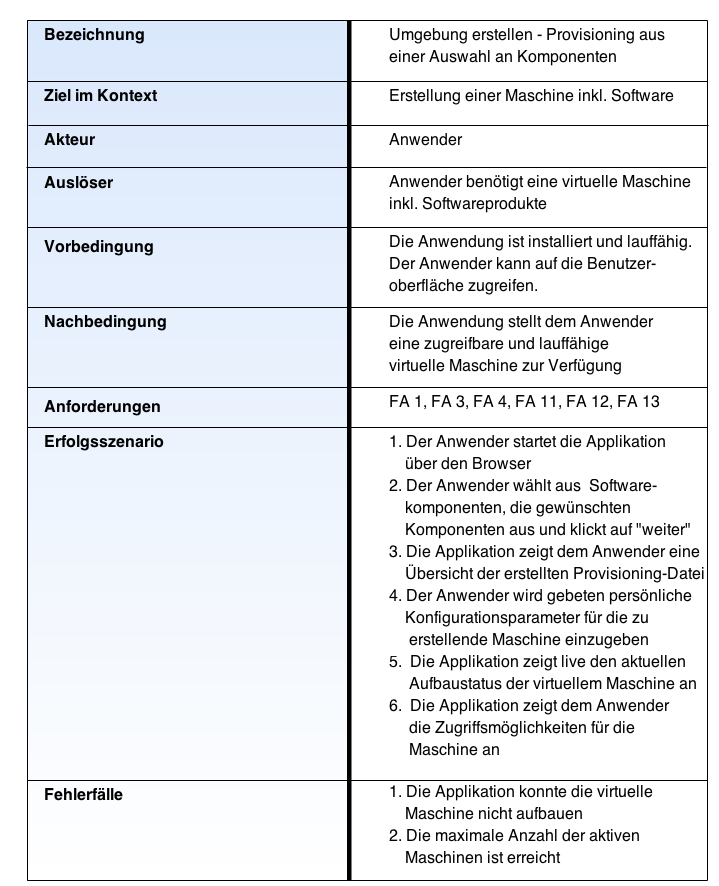
\includegraphics[scale=0.4]{../Bilder/usecase_provisioning.png}
	\captionof{figure}[kurze Bildunterschrift]{Bildunterschrift}
 \end{minipage}
\end{center}

Anforderungen: [12312312312312312312]\newline


\textbf{Anwendungsfall AF 2}
\begin{center}
 \begin{minipage}{\linewidth}
	\centering
	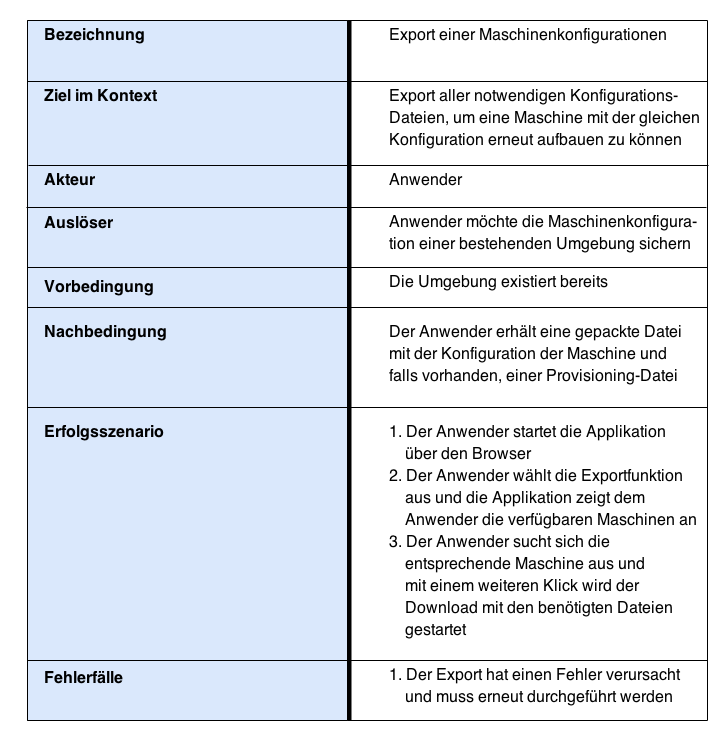
\includegraphics[scale=0.4]{../Bilder/usecase_export.png}
	\captionof{figure}[kurze Bildunterschrift]{Bildunterschrift}
 \end{minipage}
\end{center}

Anforderungen: [12312312312312312312]\newline

\textbf{Anwendungsfall AF 3}
\begin{center}
 \begin{minipage}{\linewidth}
	\centering
	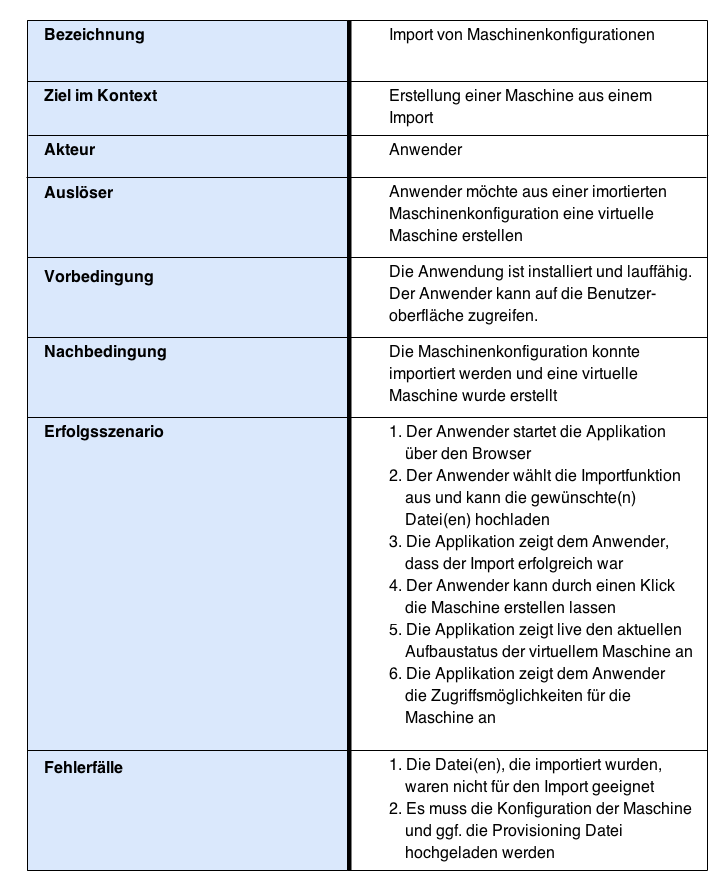
\includegraphics[scale=0.4]{../Bilder/usecase_import.png}
	\captionof{figure}[kurze Bildunterschrift]{Bildunterschrift}
 \end{minipage}
\end{center}

Anforderungen: [12312312312312312312]\newline

\section{Randbedingungen}

\subsection{Technische Randbedingungen}
\begin{center}
 \begin{minipage}{\linewidth}
	\centering
	\includegraphics[scale=0.6]{../Bilder/technische_randbedingungen.png}
	\captionof{figure}[kurze Bildunterschrift]{Bildunterschrift}
 \end{minipage}
\end{center}




\subsection{Organisatorische Randbedingungen}	

\section{Zusammenfassung}